\documentclass[amsmath, preprintnumbers, 10pt, onecolumn, pre,longbibliograpy, notitlepage]{revtex4-1}
%\documentclass[amsmath, preprint, 12pt, onecolumn, prl,longbibliograpy]{revtex4-1}

\usepackage{graphicx}
\usepackage{subfigure}

\newcommand{\MW}{\mathbf W}
\newcommand{\MB}{\mathbf B}
\newcommand{\MA}{\mathbf A}
\newcommand{\MX}{\mathbf X}
\newcommand{\MZ}{\mathbf Z}
\newcommand{\Malpha}{\mathbf\alpha}
\newcommand{\aff}{\mathcal A}
\newcommand{\R}{\mathcal R}
\newcommand{\N}{\mathcal N}
\newcommand{\vP}{\mathbf P}
\renewcommand{\Re}{{\mathrm Re}}
\renewcommand{\Im}{{\mathrm Im}}
\usepackage{physics}

\begin{document}
\title{Supplementary Material: High chemical affinity increases the robustness of biochemical oscillations}
\author{Clara \surname{del Junco} and Suriyanarayanan Vaikuntanathan}
\affiliation{Department of Chemistry and The James Franck Institute, University of Chicago, Chicago, IL, 60637}

\maketitle

\section{The first non-zero eigenvalue as an approximation of the number of coherent oscillations and period of oscillations}

In a system such as the one pictured in Fig.~1 of the main text, we can define correlation function $C_{11}(t)$ as the conditional probability of the system being in state 1 at time $t$ given that it began in state 1 at time 0. It is given by the solution of the master equation:
 \begin{align}
 C_{11}(t) & \equiv [\exp(\MW t)\mathbf P (0)]_1 \\
 &= \sum_{j=0}^{N-1} P_j^{ss} e^{\phi_j t}  \label{eq:c11sum} \\
 & =  \sum_{j=0}^{N-1} P_j^{ss} \exp[- \Re[\phi_j] t] (\cos[\Im[\phi_j] t] + i\sin[\Im[\phi_j] t])
 \label{eq:c11}
 \end{align}
where ${\phi_j}$ are the $N$ eigenvalues of the $N \times N$ matrix $\MW$, $P_j^{ss}$ is the steady-state probability of finding the system in state $j$, and $[...]_1$ is the first element of the vector.

To see why the first non-zero eigenvalue $\phi_1$, which we simply denote $\phi$ in the main text, is sufficient to approximate the number of coherent oscillations, we begin with the uniform case. In that case, Eq.~\ref{eq:c11sum} simplifies to:
\begin{equation}
 C_{11}(t) =  \frac{1}{N} \sum_{j=0}^{N-1}e^{\phi_j t} 
\end{equation}

As noted in the main text and illustrated in Fig.~\ref{fig:evspectrumuniform}, the transition rate matrix $\MW_0$ for this system is a circulant matrix whose eigenvalues lie in an ellipse in the complex plane with semi-major axis $a = k^+ + k^-$ and semi-minor axis $b=k^+ - k^-$ centered on the point $(-a, 0)$. When the affinity is large and $k^+/k^- \gg 1$, this effectively becomes a circle of radius $r = k^+$ centered at $(-r, 0)$.

 The first eigenvalue is $\phi_0$ = 0, so the first term of the sum in Eq.~\ref{eq:c11sum} gives a constant contribution of $1/N$. The angle from the real axis to the $j$th eigenvalue $\phi_j$ is $2\pi j/N$. The imaginary part of $\phi_j$ is given by $r\sin(2\pi j/N)$, and the period of oscillations of the $m$th term in Eq.~\ref{eq:c11} is $T_j = 2\pi/(r\sin(2\pi j/N))$. The ratio of $T_1$ from the first non-zero eigenvalue to $T_j$ from any subsequent eigenvalue is:
\begin{equation}
\frac{T_j}{T_1} = \frac{\sin(2\pi/N)}{\sin(2\pi j/N)} \approx \frac{2\pi/N}{2\pi j/N} = \frac{1}{j}
\end{equation}
for $N \gg j$. 
The total period of the oscillations is therefore always $T_1$. Since $\Re[\phi_1] < \Re[\phi_j]$ for all $j>1$, the number of oscillations of the correlation function $\N$ is given exactly by $|\Im[\phi_1]| /(-2\pi \Re[\phi_1]) =  \R/2\pi$. Moreover, by the same reasoning the ratio of decay times $\tau_j/\tau_1$ where $\tau_i = -1/\Re[\phi_j]$ is ~$j^2$, so oscillations due to the second eigenvalue are damped out four times faster than the first, and the $j = 1$ term is the only important oscillating contribution to $C_{11}(t)$ for after a transient period.

\begin{figure}
\centering
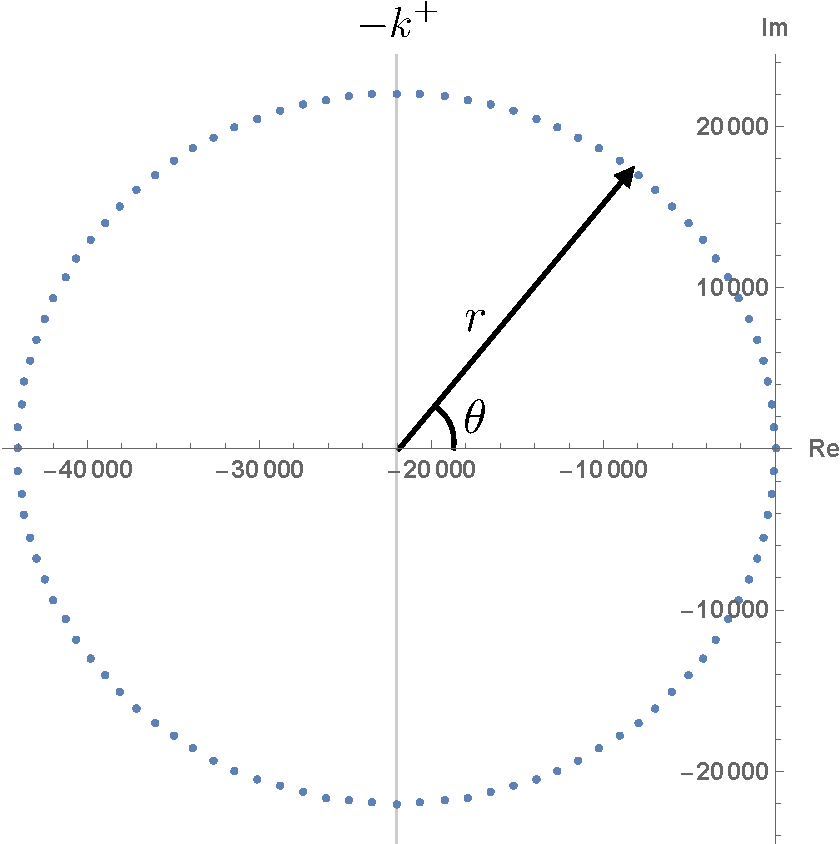
\includegraphics[width = 0.3\linewidth]{si-fig1.pdf}
\caption{Eigenvalues of a circulant matrix representing a network of size $N = 100$ with uniform rates $k^+ = e^{10}$ and $k^- = 1$.}
\label{fig:evspectrumuniform}
\end{figure}

When defects are added the eigenvalues will no longer lie on a perfect circle in the plane, and the arguments above will no longer hold exactly. For small perturbations (1 or 2 defect rates) it is reasonable to assume that the eigenvalues will not change very much and that $\R/2\pi \approx \N$. However, for large amounts of disorder it is not obvious that this will still be the case. $T_j/T_1$ may no longer be an integer, so that the total period of oscillations $T\neq T_1$, and moreover the period of the oscillations at short times ($T(1)$) and the period of oscillations at long times ($T(\tau)$) may not be the same. While $T(\tau)$ should be close to $T_1$, since all other contributions will have been damped out, $T(1)$ may not be. Yet, if the oscillator needs to be tuned to have the same period as an external signal to which it is entrained, $T_1$ (or $T_j$ where $j$ is a small integer) is likely to be the most relevant timescale.

%From Eq.~3 and 4 in the main text, we know that the real part of the first order perturbation to the first non-zero eigenvalue is on the order of $m/N^2$, and the imaginary part is on the order of $m/N$ where $m$ is the number of defects. This implies:
%\begin{align}
%\frac{T_j}{T_1}  &\approx \frac{r2\pi/N + \mathcal O(m/N)}{r2\pi m/N + \mathcal O(N_d/N)}  \\
%\frac{\tau_j}{\tau_1} &\approx \frac{r(2\pi/N)^2 + \mathcal O(N_d/N^2)}{r(2\pi m/N)^2 + \mathcal O(N_d/N^2)}.
%\end{align}
%
%Thus, the approximations $\R \approx 2\pi \N$ and $T_1 \approx T(\tau) \approx T(1)$ will improve with increasing value of $2\pi r/N_d = 2\pi k^- \exp(\aff/N)/N_d$. For example, for 20 defects in a network of size $N = 100$, this ratio is equal to about 2.5 for $\aff/N = 2$ and about 7000 for $\aff/N = 10$. Even though this is a very rough approximation, it shows that we should expect the approximations $\R \approx \N$ and $T_1 \approx T(\tau) \approx T(1)$ to improve with decreasing number of defects (which is intuitive) and increasing $\aff$. 
In Fig.~\ref{fig:periodhistograms} we show histograms of the relative difference $(T(1) - T_1)/T(1)$ for different realization of matrices of size $N = 100$ with reverse rates all equal to 1, random forward rates $h_i^+$  chosen from a Gaussian distribution with mean $\mu = \exp(\aff/N)$ and variance $\sigma^2 = 0.25 \exp(\aff/N) $, and uniform forward rates $k^+$ set to maintain a constant $\aff$. We emphasize that here we are considering the difference between the first term of Eq.~\ref{eq:c11sum} and the full correlation function, both of which are obtained by numerical diagonalization. The theory presented in the main text is another level of approximation of $T_1$ on top of this.

\begin{figure}
\centering
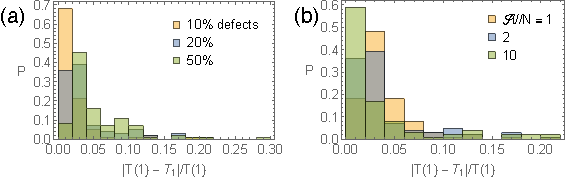
\includegraphics[width = 0.7\linewidth]{si-fig2.pdf}
\caption{Histograms of the relative difference between the first period of oscillations of the correlation function $C_{11}(t)$ ($T(1)$) and the period of oscillations due to the first eigenvalue  $T_1 = 2\pi/\Im[\phi]$. $T(1)$ is the location of the first peak of $C_{11}(t)$ obtained by exponentiating the full transition rate matrix. $T_1$ was calculated from the first eigenvalue, which was also obtained numerically. The data for each set of parameters were obtained from 100 randomly generated matrices (a) At constant $\aff/N = 2$ The agreement between $T(1)$ and $T_1$ gets worse with increasing disorder. (b) With the percent of defects held constant at 20\%, the agreement between $T(1)$ and $T_1$ improves with increasing $\aff/N$.}
\label{fig:periodhistograms}
\end{figure}

\section{Detailed calculations}

%By rearranging each of the eigenvalue equations $\MW_0 \mathbf f = \phi^{(0)}\MW_0$ where $\mathbf f$ is the eigenvector corresponding to $\phi^{(0)}$, we can recast the eigenvalue equation as:
%\begin{equation}
%\begin{bmatrix}
%f_2 \\ f_1
%\end{bmatrix}
%=
%\MB^{N}
%\begin{bmatrix}
%f_2 \\ f_1
%\end{bmatrix}
%\label{eq:BN}
%\end{equation}
%where 
%\begin{align}
%\MB &= 
%\begin{bmatrix}
%\frac{\phi^{(0)}+ k^- + k^+}{k^+} & - \frac{k^-}{k^+} \\
%1 & 0
%\end{bmatrix}\label{eq:bmatrix}\end{align}
%
%$\mathbf B$ maps the eigenvector magnitudes $(f_{i-1}, f_i)$ to $(f_i, f_{i+1})$~\cite{Vaikuntanathan2014a}.
%
%Since $\MB^N$ must have an eigenvalue of 1 according to Eq.~\ref{eq:BN}, this gives us an alternative to the eigenvalue equation for finding $\phi^{(0)}$.
%Now we consider the effect of changing the rates along $m$ links of the network from $k^{\pm}$ to $h_j^{\pm}$ - we refer to $h_j^\pm$ as a `defect rate'. Without loss of generality, we assume that the first defect rates in the network are on either side of state 1. We place the second set of defects around the state located a distance $L_1 \geq 1$ from state 1, and so forth. The product of transfer matrices in Eq.~\ref{eq:BN} becomes:
%\begin{equation}
%\begin{bmatrix}
%f_2 \\ f_1
%\end{bmatrix}
%=
%\MA_{1}\MB^{L_1}\cdots \MA_{j}\MB^{L_j} \cdots \MA_{m}\MB^{L_m}
%\begin{bmatrix}
%f_2 \\ f_1
%\end{bmatrix}
%\label{eq:AB}
%\end{equation}
%where the $A_{j}$ matrices are the same as $\MB$ but with $k^\pm$ replaced by $h_j^\pm$, and $\sum_{j=1}^m L_j = N-m$. In modifying the network in this manner we have changed the eigenvalues of $\MW$, so that $\MB$ is no longer a function of $\phi^{(0)}$ but of a new $\phi$. We assume that the perturbed value of $\phi$ has the form:
%\begin{equation}
%\phi = \phi^{(0)} + C\gamma/N + \mathcal O(1/N^2) \equiv \phi^{(0)} + \phi^{(1)} + \mathcal O(1/N^2).
%\label{eq:phipert}
%\end{equation}
%where $C$ is a constant that we choose for convenience. Inserting Eq.~\ref{eq:phipert} in to Eq.~\ref{eq:bmatrix} we obtain $\MB = \MB_0 + \MB_1$ where $\MB_1 = \{\{C\gamma/(Nk^+), 0\},\{0, 0\}\}$.  We can now find the eigenvalues $\beta_{i}$ of $\MB$ using the usual first-order eigenvalue perturbation expression \cite{Vaikuntanathan2014a, Marcus2001}. We obtain:
%\begin{align}
%\beta_1 &= \beta_1^{(0)} + \beta_1^{(1)} = e^{-2\pi i/N} (1 + \frac{\gamma}{N}) \approx e^{(-2\pi i + \gamma)/N} \label{beta1}\\
% \beta_2 &\approx \frac{k^-}{k^+}e^{(2\pi i + \gamma)/N}  = e^{-\aff/N}e^{(2\pi i + \gamma)/N} < 1\label{beta2} 
%\end{align}
%
%We can then approximate $\MB^{L_j}$ using the first-order eigenvalues and zero-order eigenvectors of $\MB$:
%\begin{align}
%&\MB^{L_j} = \sum_i \beta_i^{L_j} \MX_i % \approx  \beta_1^{L_j} \MX_1^{(0)}
%\label{eq:btoL}
%\end{align} 
%where $\MX_i$ is the the outer product of the $i$th eigenvector of $\MB$ ($\ket{i}\bra{i}$). Plugging this back in to Eq.~\ref{eq:AB} yields an expression with terms that depends on all of the values of the defect rates ($h_j^\pm$) as well as their spacings ($L_j$) and the order in which they appear. However, since $\beta_2 \propto e^{-\aff/N} < 1$, we can see that if $e^{-\aff L_j/N}$ is sufficiently small, all of the terms containing $\beta_2$ will vanish. In this limit, combining Eq.~\ref{eq:AB} and~\ref{eq:btoL}, we get:
%\begin{align}
%\begin{bmatrix}
%f_2 \\ f_1
%\end{bmatrix}
%=
%\beta_1^{N-2m}\prod_{j=1}^m \mathbf Z_j
%\begin{bmatrix}
%f_2 \\ f_1
%\end{bmatrix}
%&& \mathbf Z_j  \equiv \MA_{j}\MX_1^{(0)}
%\label{eq:ABreduced}
%\end{align}
%
%We can now compute the matrix product in Eq.~\ref{eq:ABreduced} and set its eigenvalue equal to 1 in order to solve for $\phi$. In principle, the order of the matrices in the matrix product in Eq.~\ref{eq:ABreduced} is important and hence the values of $\phi$ and $\R$ depend on the order of the defects. However, our calculations are simplified due to a special symmetry in the $\mathbf Z_j$ matrices, which have the form:  
%\begin{equation}
%\begin{bmatrix}
%c_j a & c_j b \\
%a & b
%\end{bmatrix}\,,
%\end{equation}
%where the specific algebraic expressions for $c_j$, $a$, and $b$ are provided in SM Eq.~29-31~\cite{Supplemental}. These matrices have two properties that are relevant here: first, since the two rows of $\mathbf Z_j$ are related by a constant, $\mathbf Z_j$ has a zero eigenvalue. Second, the eigenvalue of the product $\mathbf Z_i \mathbf Z_j$ is the product of the eigenvalues of $\mathbf Z_i$ and $\mathbf Z_j$. 
%Given these two properties, the expression for $\phi$ is simply determined by the non-trivial eigenvalue of the product of $\mathbf Z_j$ matrices which in turn is simply equal to the product of the non-trivial eigenvalue of the $\mathbf Z_j$ matrices. The order in which the defects are placed, the spacing between them, or any other higher order correlation hence becomes irrelevant as far as $\phi$ is concerned. Specifically, for a network of size $N$ with $m$ defects at any positions we find:

\subsection{Transfer matrix formulation}

To find the first non-zero eigenvalue $\phi$ of the transition matrix $\MW$ in the disordered system, %we could perform a standard eigenvalue perturbation theory on $\MW$. However, this approach restricts us to changing the entries of $\MW$ by only a small amount.  To circumvent this, 
we will take advantage of the local nature of connections in this system to recast the eigenvalue problem in terms of transfer matrices.

Consider the eigenvalue equation for the circulant matrix $\MW_0$:
\begin{equation}
 \begin{bmatrix} 
    -(k^- + k^+) & k^- & \dots &  k^+ \\
    k^+ &  -(k^- + k^+) & k^- & \dots \\
    \vdots &  & \ddots & \\
    k^- &  \dots  &  k^+  &  -(k^- + k^+) \\
    \end{bmatrix}
     \begin{bmatrix} 
   f_1 \\ f_2 \\ \vdots \\ f_N
    \end{bmatrix}
    = \phi^{(0)}
         \begin{bmatrix} 
   f_1 \\ f_2 \\ \vdots \\ f_N
    \end{bmatrix}
    \label{eq:transfer_step1}
\end{equation}
We can then write:
\begin{align}
-(k^- + k^+)f_1 + k^-f_2 + k^+f_N &= \phi^{(0)} f_1\\
 -(k^- + k^+)f_2 + k^-f_3 + k^+f_1 &= \phi^{(0)} f_2  \label{eq:transfer_step2}
\end{align}
and so forth, with 
\begin{equation}
\phi^{(0)} = -(k^- + k^+) + k^-\exp(-2 \pi i/N) + k^+\exp(2 \pi i/N).
\end{equation}
Solving for $f_1$ in Eq.~\ref{eq:transfer_step2} gives:
\begin{equation}
f_1 = \frac{\phi^{(0)}+ k^- + k^+}{k^+} f_2 - \frac{k^-}{k^+}f_3
\label{eq:transfer_step3}
\end{equation}
which we can also write as:
\begin{equation}
\begin{bmatrix}
f_1 \\ f_2
\end{bmatrix}
= 
\begin{bmatrix}
\frac{\phi^{(0)}+ k^- + k^+}{k^+} & - \frac{k^-}{k^+} \\
1 & 0
\end{bmatrix}
\begin{bmatrix}
f_2 \\ f_3
\end{bmatrix}
\equiv
\mathbf B 
\begin{bmatrix}
f_2 \\ f_3
\end{bmatrix}
\label{eq:transfer_step4}.
\end{equation}
Thus, $\mathbf B$ maps the eigenvector magnitudes $(f_{i-1}, f_{i})$ to $(f_{i}, f_{i+1})$. Because the matrix $\mathbf B$ is the same for each link in the unicyclic network with uniform rates, we have:
\begin{equation}
\begin{bmatrix}
f_1 \\ f_2
\end{bmatrix}
=
\mathbf B^N
\begin{bmatrix}
f_1 \\ f_2
\end{bmatrix}
\label{eq:transfer_step5}
\end{equation}
so that $\mathbf B^N$ must have an eigenvalue of 1.  Solving for the eigenvalues of $\mathbf B^N$ will give a polynomial of order $(\phi^{(0)})^N$, the $N$ roots of which are the $N$ eigenvalues of the transition matrix $\MW_0$. This gives us an alternative to Eq.~\ref{eq:transfer_step1} for finding $\phi^{(0)}$.

\subsection{One defect rate}

We first consider the case of adding one set of ``defect" rates $h^\pm$. To do so we replace one of the $\mathbf B$ matrices in the product in Eq.~\ref{eq:transfer_step5} by
\begin{equation}
\MA \equiv 
\begin{bmatrix}
\frac{\phi+ h^- + h^+}{h^+} & - \frac{h^-}{h^+} \\
1 & 0
\end{bmatrix}.
\end{equation}
which maps the eigenvector elements on either side of the link with the defect rates. The new product of transfer matrices is:
\begin{equation}
\begin{bmatrix}
f_1 \\ f_2
\end{bmatrix}
=
\MA \MB^{N-1}
\begin{bmatrix}
f_1 \\ f_2
\end{bmatrix}.
\label{eq:AB}
\end{equation}
Now the $\mathbf B$ matrix has changed, since modifying the rates changes the value of $\phi$. We write $\phi$ in the most general way as:
\begin{equation}
\phi = \phi^{(0)} + C\gamma
\label{eq:phipert}
\end{equation}
where $C$ is a constant to be determined, which implies 
\begin{equation}
\MB = \MB_0 + \begin{bmatrix} C\gamma/(k^+) &  0 \\ 0 & 0 \end{bmatrix} \equiv \MB_0 + \MB_1
\end{equation}
with $\MB_0$ given by equation \ref{eq:transfer_step4}.

We now proceed with the matrix perturbation of $\mathbf B$. First we compute the eigenvalues ($\beta_i$) and normalized eigenvectors of $\mathbf B_0$. Note that since $\mathbf B_0$ is non-Hermitian, its right and left eigenvectors ($\bra{i}$ and $\ket{i}$) are not the same and we need to compute them separately in order to get an orthonormal basis set~\cite{Marcus2001}. The left eigenvectors of $\mathbf B_0$ are the right eigenvectors of $\mathbf B_0^\dagger$ (the conjugate transpose of $\mathbf B_0$). We obtain:
\begin{align}
\beta_1^0&= e^{2\pi i/N} &&\beta_2^0 = (k^-/k^+)e^{-2\pi i/N} \\
\ket{1_0} &= \frac{1}{c_1}(e^{2\pi i/N}, 1) &&\ket{2_0} =\frac{1}{c_2}((k^-/k^+)e^{-2\pi i/N}, 1) \\
\bra{1_0} &= \frac{1}{c_1}(-(k^+/k^-)e^{2\pi i/N}, 1) && \bra{2_0} = \frac{1}{c_2}(-e^{-2\pi i/N},1) \\
c_1^2 & = 1-(k^+/k^-)e^{4\pi i/N}  && c_2^2 = 1 - (k^-/k^+)e^{-4\pi i/N}
\end{align}
(it is easy to verify that this is an orthonormal basis set).
Now we compute the first-order correction to the eigenvalues:
\begin{equation}
\beta_1^{(1)} = \mel{1_0}{\mathbf B_1}{1_0} =-\frac{e^{4\pi i /N}}{c_1^2}\frac{C\gamma}{k^-}.
\label{eq:PT1}
\end{equation}
We choose
\begin{equation}
C = -c_1^2 k^- e^{-2\pi i/N}
\label{eq:constant}
\end{equation}
so that
 \begin{equation}
 \beta_1^{(1)} = e^{2\pi i/N}\gamma
 \end{equation}
giving
  \begin{equation}
 \beta_1 = e^{2\pi i/N} (1 + \gamma).
 \end{equation}
 Similarly,
  \begin{equation}
 \beta_2 = \frac{k^-}{k^+}e^{-2\pi i /N}(1 + \gamma) =  e^{-\aff/N}e^{-2\pi i /N}(1 + \gamma).
 \end{equation}
We can now compute $\mathbf B^{N-1}$ using:
 \begin{equation}
\mathbf B^{N-1} =\sum_i \beta_i^{N-1}\MX^{0}_i
 \end{equation}
where $\MX^{0}_i\equiv \ket{i_0}\bra{i_0}$ is the outer product of zero-order eigenvectors. Since $\beta_2 \propto e^{-\aff/N} < 1$, we can see that if $\aff$  is sufficiently large, all of the terms containing $\beta_2$ will vanish. Then, Eq.~\ref{eq:AB} reduces to:
\begin{equation}
\begin{bmatrix}
f_1 \\ f_2
\end{bmatrix}
=
\beta_1^{N-1}\MA \MX_1^{(0)}
\begin{bmatrix}
f_1 \\ f_2
\end{bmatrix}
\label{eq:ABreduced}
\end{equation}
where $\MX_1^{(0)}$ is:
\begin{equation}
\MX_1^{(0)}
 = \frac{1}{c_1^2}
 \begin{bmatrix}
- e^{4\pi i /N}k^+/k^- & e^{2\pi i /N}\\
- e^{2\pi i /N}k^+/k^-  & 1
 \end{bmatrix}
\end{equation}
%We will only use the zero-order eigenvectors to compute $\mathbf B^{N-m}$:
%\begin{equation}
%\mathbf B^{N-m} = \beta_1^{N-m} \MX_1^{(0)}
% = \frac{\exp[\gamma -m\gamma/N + 2m\pi i / N]}{c_1^2}
% \begin{bmatrix}
% e^{-2\pi i /N} &  -k^-/k^+\\
%  1 & - e^{2\pi i /N}(k^-/k^+)
% \end{bmatrix}
%\end{equation}

\subsubsection{Comparing to exact eigenvalues of $\MB$}

Since $\MB$ is a two by two matrix, we can compute its exact eigenvalues and check how the error in our perturbative approximations of $\beta_1$ and $\beta_2$ scales. This will reveal what the `perturbative parameter' in our theory is. The exact eigenvalues of $\MB$ are:
\begin{align}
\beta_{\mathrm{exact}}^\pm &= \frac{e^{-2\pi i/N}}{2}\left(\frac{k^-}{k^+}(1 - \gamma) + e^{4\pi i /N}(1 + \gamma) \pm \left[-4e^{4\pi i/N}\frac{k^-}{k^+} + \left( \frac{k^-}{k^+}(1 - \gamma) + e^{4\pi i/N}(1 + \gamma) \right)^2 \right]^{1/2}\right) \\
& = \frac{e^{-2\pi i/N}}{2}\left(e^{-\aff/N}(1 - \gamma) + e^{4\pi i /N}(1 + \gamma) \pm \left[-4e^{4\pi i/N}e^{-\aff/N} + \left( e^{-\aff/N}(1 - \gamma) + e^{4\pi i/N}(1 + \gamma) \right)^2 \right]^{1/2}\right)
\label{betaexact}
\end{align}
If we ignore terms of order $e^{-\aff/N}$ compared to terms of order 1, the expressions above simplify to:
\begin{equation}
\lim_{\exp(-\aff/N) \to 0} \beta_{\mathrm{exact}}^\pm =  \frac{e^{2\pi i/N}}{2} \left( (1 + \gamma) \pm (1 + \gamma) \right)
\end{equation}
giving
\begin{align}
\lim_{\exp(-\aff/N) \to 0} \beta_{\mathrm{exact}}^+ =  e^{2\pi i/N} (1 + \gamma) = \beta_1 && \lim_{\exp(-\aff/N) \to 0} \beta_{\mathrm{exact}}^-= 0
\end{align}
In the limit of very high affinity, Eq.~\ref{eq:ABreduced} is exact. Therefore, the small parameter in our theory is $\exp(-\aff/N)$.

\subsubsection{Solving for $\gamma$}

We can now compute the matrix product in Eq.~\ref{eq:ABreduced} and set its eigenvalue equal to 1 in order to solve for $\phi$. Recall that $\MA$ is also a function of $\phi$, so we will also include $\gamma$ in $\MA$. In the case of a single defect, where $\gamma$ is small, this effect is likely to be insignificant and it would be sufficient to approximate $\MA$ as a function of $\phi^{(0)}$ only. However, below we will add multiple defects to the network and in that case, including $\gamma$ in $\MA$ is important. We find:
\begin{equation}
\MA \MX_1^{(0)} \equiv \mathbf Z  = \frac{1}{c_1^2}
\begin{bmatrix}
d a & d b \\ a & b
\end{bmatrix}
\label{eq:z}
\end{equation}
where 
\begin{align}
d(h^\pm)  &= \frac{ \gamma+e^{-2 i \pi /N} (k^--h^-) +k^+ e^{2 i \pi/N}+h^-+h^+-k^--k^+}{h^+} \\
a &= -e^{4\pi i/N}k^+/k^- \\
b & = e^{2\pi i /N}
\end{align}

Since the two rows of $\mathbf Z$ are related by a constant, $\mathbf Z$ has a zero eigenvalue. The non-trivial eigenvalue $\zeta$ of $\mathbf Z$ is:
\begin{equation}
\zeta = \frac{e^{2\pi i/N} \left({k^+} e^{2\pi i/N} (-C\gamma-{h^-}-{h^+}+{k^-}+{k^+})+{h^-} {k^+}+{h^+} {k^-}-{k^-} {k^+} -e^{4\pi i/N}{k^+}^2\right)}{c_1^2 {h^+} {k^-}}.
\label{eq:zeta}
\end{equation}
We can now solve for $\gamma$ using:
\begin{align}
1 & =\beta_1^{N-1}  \zeta \\
& = e^{-2\pi i/N} (1 +\gamma)^{N-1} \zeta
\end{align}
For notational simplicity we absorb the $e^{-2\pi i/N}$ term in to $\zeta$, letting 
\begin{equation}
\zeta' = e^{-2\pi i/N}\zeta.
\label{eq:zetaprime}
\end{equation}
Rearranging, we have:
\begin{equation}
(1 + \gamma)=  \zeta'^{1/(1-N)}
\end{equation}
We now rewrite $\zeta'^{1/(1-N)}$ as $\exp(\log(\zeta'^{1/(1-N)})) = \exp(\left(\frac{1}{1-N}\right)\log(\zeta'))$ and expand:
\begin{equation}
\exp(\left(\frac{1}{1-N}\right)\log(\zeta')) \approx 1 + \frac{1}{1-N}\log(\zeta') + \frac{1}{2(1-N)^2}(\log(\zeta'))^2+ \cdots,
\end{equation}
giving
\begin{equation}
1 + \gamma \approx 1 + \frac{1}{1-N}\log(\zeta')  + \frac{1}{2(1-N)^2}(\log(\zeta'))^2
\end{equation}
The 1's cancel and we get:
\begin{equation}
\gamma \approx  \frac{1}{1-N}\log(\zeta') + \frac{1}{2(1-N)^2}(\log(\zeta'))^2.
\label{eq:gamma-self-cons}
\end{equation}

This gives a self-consistent equation for $\gamma$ (since $\zeta'$ is a function of $\gamma$). To obtain the results in the main text, we solved eq.~\ref{eq:gamma-self-cons} numerically by searching for roots of the equation in the neighborhood of the analytical approximation that we can obtain from expanding the logarithms in eq.~\ref{eq:gamma-self-cons} to first order. To obtain this analytical approximation we rewrite $\zeta'$ as:
\begin{equation}
\zeta' = \zeta'_0 - \gamma \frac{ {k^+} e^{2\pi i/N} C}{c_1^2 {h^+} {k^-}} = \zeta'_0 - \gamma \frac{ k^+}{ h^+ }
\end{equation}
where $ \zeta'_0 $ is independent of $\gamma$.
We then expand the logarithm as:
\begin{align}
\log(\zeta') &= \log\left(\zeta'_0 - \gamma \frac{ k^+}{ h^+ }\right) \\
& = \log\left(\zeta'_0 \left(1 - \gamma \frac{ k^+}{ h^+ \zeta'_0}\right)\right)\\
& \approx \log(\zeta'_0)  - \gamma \frac{ k^+}{ h^+ \zeta'_0}
\end{align}
where in the last line we have used $\log(1 + x) \approx x$ for $x\ll 1$.  Plugging this back in to Eq.~\ref{eq:gamma-self-cons} and keeping only the term linear in $1/(1-N)$ gives:
\begin{equation}
\gamma \approx  \frac{1}{1-N}\left[\log(\zeta'_0) - \gamma \frac{ k^+}{h^+ \zeta'_0}\right].
\label{eq:gamma-expand-1}
\end{equation}
%Now, we compute $\mathbf A_1.\mathbf A_2.\mathbf B^{N-2}$ and find its eigenvalues $\zeta$:
%\begin{align}
%\zeta_1 &= 0 \\
%\zeta_2 &= \frac{e^{\frac{\gamma  (N-2)}{N}} \left(-k^+ e^{\frac{2 i \pi }{N}} (h^-+h^+-k^--k^+)+e^{\frac{4 i \pi }{N}} (k^+ (h^--k^-)+h^+ k^-)-(k^+)^2\right)}{h^+ \left(-k^++k^- e^{\frac{4 i \pi }{N}}\right)}\\
%& \equiv e^{\frac{\gamma  (N-2)}{N}} \chi
%\end{align}
%Solving for $\gamma$ using $\zeta_2 = 1$ gives $\gamma = -N \log \chi /(N-2)$, and the perturbed eigenvalue $\phi$ is:
%\begin{equation}
%\phi(k^+, k^-, h^+, h^-, N) = \phi_0 + \frac{ C \log\chi}{N - 2}
%\label{eq:phinew}
%\end{equation}

\subsection{Many Defect Rates}

Now we extend our results to the case where many ($m$) of the rates are `defects'.  The product of transfer matrices in this case is:
\begin{equation}
\begin{bmatrix}
f_1 \\ f_2
\end{bmatrix}
=
\MA_{1}\MB^{L_1}\cdots \MA_{j}\MB^{L_j} \cdots \MA_{m}\MB^{L_m}
\begin{bmatrix}
f_1 \\ f_2
\end{bmatrix}.
\label{eq:ABmult}
\end{equation}
where $L_j$ is the distance between neighboring defect rates and $\sum_j L_j = N-m$. 

\subsubsection{Defect spacing $L_j\geq 1$}

Recall that  
\begin{equation}
\mathbf B^{L_j} = \left(e^{-2\pi i/N} \left(1 +\gamma\right)\right)^{L_j} \MX^{0}_1 + \left(e^{-\aff/N}e^{-2\pi i /N}\left(1 + \gamma\right)  \right)^{L_j}  \MX^{0}_2.
\end{equation}
Generally, this means that eq.~\ref{eq:ABmult} has $2^m$ terms. However, if $e^{-L_j\aff/N}$ is sufficiently large, we can ignore $\beta_2$ as we did in the case of one defect above. Then, eq.~\ref{eq:ABmult} reduces to a single term from which we can factorize $\beta_1$, giving:
\begin{equation}
\begin{bmatrix}
f_1 \\ f_2
\end{bmatrix}
=
\beta_1^{N-m}\MA_{1}\MX_1^{(0)}\cdots \MA_{j}\MX_1^{(0)} \cdots \MA_{m}\MX_1^{(0)}
\begin{bmatrix}
f_1 \\ f_2
\end{bmatrix}
\label{eq:ABmultreduced}
\end{equation}


The affinity thus sets a correlation length for the defects; if the affinity per site ($\aff/N$) is sufficiently large, the spacing between them does not matter. In principle, the order of the matrices in the matrix product in Eq.~\ref{eq:ABmultreduced} is however still important and hence the values of $\phi$ and $\R$ depend on the order of the defects. However, our calculations are simplified due to the special symmetry of $\mathbf Z_j \equiv \MA_j\MX_1^{(0)}$ (given explicitly by Eq.~\ref{eq:z} with the defect rates $h^\pm$ now indexed $h_j^\pm$, etc.). It turns out that the non-trivial eigenvalue of the product $\mathbf Z_i \mathbf Z_j$ is the product of the non-trivial eigenvalues of $\mathbf Z_i$ and $\mathbf Z_j$.  As a result, the expression for $\phi$ is simply determined by the product of the non-trivial eigenvalues of the $\mathbf Z_j$ matrices. Therefore, as long as $L_j \geq 1 \forall j$, the order in which the defects are placed and the spacing between them becomes irrelevant as far as $\phi$ is concerned.  We can simply extend our results for one defect to write:
\begin{equation}
\gamma\approx  \frac{1}{m-N}\sum_{j=1}^m \log(\zeta_j') + \frac{1}{2(m-N)^2}\left(\sum_{j=1}^m \log(\zeta_j')\right)^2.
\label{eq:gamma-self-cons-mult}
\end{equation}
where $\zeta'_j$ is a function of $k^+, k^-, h^+_j, h^-_j, N$ given by eq.~\ref{eq:zeta} and ~\ref{eq:zetaprime} but is independent of any of the other defect rates.
The corresponding analytical approximation is:
\begin{equation}
\gamma \approx  \frac{1}{m-N}\left[\sum_{j=1}^m\log(\zeta'_{0,j}) - \gamma \frac{ k^+}{ \sum_{j=1}^mh^+_j \zeta'_{0,j}}\right].
\label{eq:gamma-expand-mult}
\end{equation}

Our derivation depends on the distance between defect rates in the networks being at least one ($L_j\geq 1$). Nonetheless, our numerical results in the main text show that these expressions accurately predict the eigenvalues of the oscillator even when $L_j = 0$ for nearly all of the defects. We now discuss how high affinity makes this possible. 

\subsubsection{Defect spacing $L_j = 0$}

The reason we require $L_j\geq 1$ is that the non-trivial eigenvalue of the product $\mathbf Z_i \mathbf Z_j$, where $\mathbf Z_j \equiv \MA_j\MX_1^{(0)}$, is the product of the non-trivial eigenvalues of $\mathbf Z_i$ and $\mathbf Z_j$.  However, the eigenvalue of the product of $\MA_i\MA_j$ is $not$ the product of their eigenvalues. Therefore, Eq.~\ref{eq:gamma-self-cons-mult} should not be valid if there are defect rates on either side of the same node in the network. In this case we need to consider the products $\MA_i\MA_j$, $\MA_i\MA_j\MA_k$, etc., for clusters of 2, 3, etc. defects. We find that the matrices
\begin{align}
\MZ_{2}^{ij} &\equiv \MA_j  \MA_i\MX_1^{(0)} \\
\MZ_{3}^{ijk} &\equiv \MA_j  \MA_i \MA_k\MX_1^{(0)}\\
\cdots \\
\MZ_{m}^{ij\cdots } &\equiv \MA_j  \MA_i \cdots \MA_m \MX_1^{(0)}
\end{align}
have the same properties as the $\MZ$ matrices, i.e. the eigenvalue of the product $\prod \MZ_{m}^{ij\cdots } \MZ_{n}^{kl \cdots }$ is the product of the eigenvalues of $ \MZ_{m, ij\cdots m}$ and $\MZ_{n, kl \cdots n}$. Clearly there is a way of including higher and higher order correlations, but as soon as we include $any$ coupling of the defects we need a lot more information about their positions. In order for the defects to be completely decoupled from one another, as indeed we find that they are even at moderate affinities $\aff/N \approx 2$, we need the eigenvalue of the product of $\MA_i\MA_j$ to be the product of their eigenvalues. 
Let us write $\MA_j$ as
\begin{equation}
\MA_j = \begin{bmatrix}
x_j & - y_j \\
1 & 0
\end{bmatrix}
\end{equation}
where 
\begin{align}
x_j = \frac{\phi+ h_j^- + h_j^+}{h_j^+}  = \frac{ h_j^-e^{-2\pi i/N} + h_j^+e^{-2\pi i/N} + C\gamma/N}{h_j^+} && y_j = \frac{h_j^-}{h_j^+}
\end{align}
In the limit of large $N$, we have:
\begin{align}
\lim_{N\to \infty} x_j = \frac{ h_j^- + h_j^+ }{h_j^+} = 1 + \frac{h_j^-}{h_j^+} && y_j = \frac{h_j^-}{h_j^+}.
\end{align}
The eigenvalues of $\MA_j $ are 
\begin{equation}
\alpha^j_1 = \frac{1}{2} \left(\sqrt{{x_j}^2+4 {y_j}}+{x_j}\right), \alpha^j_2 = 0.
\end{equation}
The eigenvalues of the product $\MA_j \MA_i$ are:
\begin{align}
\alpha^{ij}_1 &= \frac{1}{2} \left(-\sqrt{({x_i} {x_j}+{y_i}+{y_j})^2-4 {y_i} {y_j}}+{x_i} {x_j}+{y_i}+{y_j}\right)\\
\alpha^{ij}_2 &= \frac{1}{2} \left(\sqrt{({x_i} {x_j}+{y_i}+{y_j})^2-4 {y_i} {y_j}}+{x_i} {x_j}+{y_i}+{y_j}\right)
\label{eq:evpair}
\end{align}
If we can ignore the $y$ terms compared to the $x$ terms, then these reduce to:
\begin{align}
\lim_{y/x \to 0}\alpha^{ij}_1 &=0\\
\lim_{y/x \to 0}\alpha^{ij}_2 &= {x_i} {x_j}
\label{eq:evpair}
\end{align}
and the eigenvalues of $\MA_i$ become $\alpha^j_1 = x_j, \alpha^j_2 = 0$. Clearly, in this limit the eigenvalue of the product of transfer matrices is equal to the product of eigenvalues, as required, and the order of the defects will no longer matter even if they are adjacent.  The limit is fulfilled when the affinity is high so that $h^-/h^+ \sim\exp(-\aff/N)$.

Following the derivation above using $x_j$ as the eigenvalue for the defect transfer matrices, we obtain the same result as in eqs.~\ref{eq:gamma-self-cons-mult} and \ref{eq:gamma-expand-mult} with $\zeta$ replaced by $x$. Indeed, we see that in the limit that $h^-/h^+\to 0$ and $k^-/k^+\to 0$, $\zeta$ reduces to $x$. This explains how our theory can handle many adjacent defects.
\pagebreak

\section{Constant affinity results}

\begin{figure}[h!]
\centering
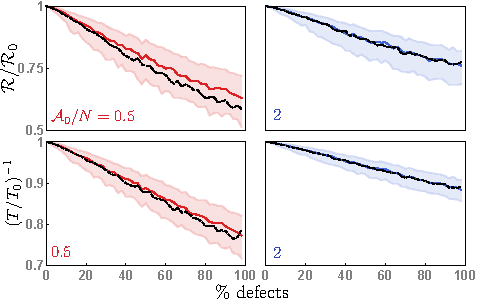
\includegraphics[width = 0.5\linewidth]{si-fig3.pdf}
\caption{Coherence $\R$ and period $T$ of an oscillator with $N = 100$ states as a function of the percent of defect rates. All counterclockwise rates are set to 1. We restrict ourselves to even numbers of defect rates. Half of the clockwise defect rates $\{h_j^+\}$ are drawn from a Gaussian distribution with mean $k^+ =  \exp(\aff_0/N)$ and standard deviation $0.4k^+$, and with a lower cutoff at 0.1 so that we do not select rates that are very close to zero or negative. We set the other half of the defect rates to $\{\exp(\aff_0/N)^2/h_j^+\}$. This prescription ensures that the affinity remains constant and equal to $\aff_0$, while also allowing the rates to vary over at least an order of magnitude.  Red curves are for $\aff_0/N = 0.5$; blue curves $\aff_0/N = 2$. Because the distributions of $\R$ and $T$ are asymmetric, rather than plotting the mean and standard deviation of the data we plot the median (solid line) $\pm$ one quartile (shaded region) of the numerical values for 500 samples of defect rates. The dashed lines are the median theoretical predictions for 500 samples of defect rates. Our results confirm the bound in Ref.~\cite{Barato2017}, as the value of $\R/\R_0$ is never greater than 1. For $\aff_0/N = 2$, our theory is accurate even when \% defects $\approx 100$. Our results confirm the bound in Ref.~\cite{Barato2017}, as the value of $\R/\R_0$ is never greater than 1, and show that $\R$ and $T$ become more robust (spread of values decreases) and predictable at high affinity.}
\label{fig:rtvsm-constaff}
\end{figure}

%\bibliography{/Users/claradeljuncooffice/Documents/library}

%merlin.mbs apsrev4-1.bst 2010-07-25 4.21a (PWD, AO, DPC) hacked
%Control: key (0)
%Control: author (8) initials jnrlst
%Control: editor formatted (1) identically to author
%Control: production of article title (-1) disabled
%Control: page (0) single
%Control: year (1) truncated
%Control: production of eprint (0) enabled
\begin{thebibliography}{2}%
\makeatletter
\providecommand \@ifxundefined [1]{%
 \@ifx{#1\undefined}
}%
\providecommand \@ifnum [1]{%
 \ifnum #1\expandafter \@firstoftwo
 \else \expandafter \@secondoftwo
 \fi
}%
\providecommand \@ifx [1]{%
 \ifx #1\expandafter \@firstoftwo
 \else \expandafter \@secondoftwo
 \fi
}%
\providecommand \natexlab [1]{#1}%
\providecommand \enquote  [1]{``#1''}%
\providecommand \bibnamefont  [1]{#1}%
\providecommand \bibfnamefont [1]{#1}%
\providecommand \citenamefont [1]{#1}%
\providecommand \href@noop [0]{\@secondoftwo}%
\providecommand \href [0]{\begingroup \@sanitize@url \@href}%
\providecommand \@href[1]{\@@startlink{#1}\@@href}%
\providecommand \@@href[1]{\endgroup#1\@@endlink}%
\providecommand \@sanitize@url [0]{\catcode `\\12\catcode `\$12\catcode
  `\&12\catcode `\#12\catcode `\^12\catcode `\_12\catcode `\%12\relax}%
\providecommand \@@startlink[1]{}%
\providecommand \@@endlink[0]{}%
\providecommand \url  [0]{\begingroup\@sanitize@url \@url }%
\providecommand \@url [1]{\endgroup\@href {#1}{\urlprefix }}%
\providecommand \urlprefix  [0]{URL }%
\providecommand \Eprint [0]{\href }%
\providecommand \doibase [0]{http://dx.doi.org/}%
\providecommand \selectlanguage [0]{\@gobble}%
\providecommand \bibinfo  [0]{\@secondoftwo}%
\providecommand \bibfield  [0]{\@secondoftwo}%
\providecommand \translation [1]{[#1]}%
\providecommand \BibitemOpen [0]{}%
\providecommand \bibitemStop [0]{}%
\providecommand \bibitemNoStop [0]{.\EOS\space}%
\providecommand \EOS [0]{\spacefactor3000\relax}%
\providecommand \BibitemShut  [1]{\csname bibitem#1\endcsname}%
\let\auto@bib@innerbib\@empty
%</preamble>
\bibitem [{\citenamefont {Marcus}(2001)}]{Marcus2001}%
  \BibitemOpen
  \bibfield  {author} {\bibinfo {author} {\bibfnamefont {R.~A.}\ \bibnamefont
  {Marcus}},\ }\href {\doibase 10.1021/jp004164d} {\bibfield  {journal}
  {\bibinfo  {journal} {J. Phys. Chem. A}\ }\textbf {\bibinfo {volume} {105}},\
  \bibinfo {pages} {2612} (\bibinfo {year} {2001})}\BibitemShut {NoStop}%
\bibitem [{\citenamefont {Barato}\ and\ \citenamefont
  {Seifert}(2017)}]{Barato2017}%
  \BibitemOpen
  \bibfield  {author} {\bibinfo {author} {\bibfnamefont {A.~C.}\ \bibnamefont
  {Barato}}\ and\ \bibinfo {author} {\bibfnamefont {U.}~\bibnamefont
  {Seifert}},\ }\href {\doibase 10.1103/PhysRevE.95.062409} {\bibfield
  {journal} {\bibinfo  {journal} {Phys. Rev. E}\ }\textbf {\bibinfo {volume}
  {95}},\ \bibinfo {pages} {062409} (\bibinfo {year} {2017})}\BibitemShut
  {NoStop}%
\end{thebibliography}%



\end{document}